\documentclass[]{article}
\usepackage{amsmath}
\usepackage{graphicx}
\graphicspath{.}

%opening
\title{ELEC 7500 Project 3}
\author{Matthew Boler}

\begin{document}

\maketitle

\section{Linear System Stability}
Assess the stability of the system $\dot{x} = \mathbf{A}_ix$ for each of the following cases.
In each case, explain whether the system is stable, asymptotically stable, or unstable.

\begin{align*}
	\mathbf{A}_1 &= \begin{bmatrix}
	0 & 1 & 0 \\
	0 & 0 & 1 \\
	-15 & -23 & -9
	\end{bmatrix} \\
	\mathbf{A}_2 &= \begin{bmatrix}
	-7 & 1 & 0 \\
	-7 & 0 & 1 \\
	15 & 0 & 0
	\end{bmatrix} \\
	\mathbf{A}_3 &= \begin{bmatrix}
	0 & 1 & 0 \\
	0 & 0 & 1 \\
	0 & -15 & -8
	\end{bmatrix} \\
	\mathbf{A}_4 &= \begin{bmatrix}
	0 & 0 & 0 \\
	0 & 0 & 0 \\
	0 & 0 & -1
	\end{bmatrix} \\
	\mathbf{A}_5 &= \begin{bmatrix}
	0 & 1 & 0 \\
	0 & 0 & 0 \\
	0 & 0 & -1
	\end{bmatrix} \\
	\mathbf{A}_6 &= \begin{bmatrix}
	0 & 1 & 0 \\
	1 & 0 & 0 \\
	0 & 0 & -1
	\end{bmatrix}
\end{align*}

\subsection{1}

The eigenvalues of this system are $\lambda_{1,2,3} = -1, -2, -3$.
As $Re(\lambda) < 0 \forall \lambda$, the system is asymptotically stable.

\subsection{2}
The eigenvalues of this system are $\lambda_{1,2,3} = 1, -3, -5$.
Since there is an eigenvalue in the right half-plane, the system is unstable.

\subsection{3}
The eigenvalues of this system are $\lambda_{1,2,3} = 0, -3, -5$.
Since there is a unique eigenvalue on the imaginary axis and the rest have negative real parts, the system is stable.

\subsection{4}
The eigenvalues of this system are $\lambda_{1,2,3} = 0,0,-1$.
As there are repeated roots on the imaginary axis, the system is unstable.

\subsection{5}
The eigenvalues of this system are $\lambda_{1,2,3} = 0,0,-1$.
As there are repeated roots on the imaginary axis, the system is unstable.

\subsection{6}
The eigenvalues of this system are $\lambda_{1,2,3} = -1, -1, 1$.
As there is an eigenvalue in the right half-plane, the system is unstable.

\section{Stable and Unstable Subspaces}

Consider the model $\dot{x} = \mathbf{A}_5x$.
Do the following:
\begin{itemize}
	\item Find basis vectors for the stable subspace and state the dimension of the subspace.
	\item Find basis vectors for the unstable subspace and state the dimension of the subspace.
	\item Characterize all initial states $x^*(0)$ that yield asymptotically stable state response for time $t \ge 0$.
	\item Verify the answer by deriving the state response $x(t) = e^{\mathbf{A}_5t}x^*(0)$ for $t \ge 0$.
\end{itemize}

The eigenvalues and their corresponding eigenvectors are as such:
\begin{align*}
	\lambda_1 &= 0, e_1 = \begin{bmatrix}
	1 \\
	0 \\
	0
	\end{bmatrix}\\
	\lambda_2 &= 0, e_2 = \begin{bmatrix}
	1 \\
	1 \\
	0
	\end{bmatrix} \\
	\lambda_3 &= -1, e_3 = \begin{bmatrix}
	0 \\
	0 \\
	0.3697
	\end{bmatrix}
\end{align*}

\subsection{Stable Subspace}

From this, we can see that the vectors 
\begin{align*}
	\begin{bmatrix}
	0 \\
	1 \\
	0
	\end{bmatrix}, \begin{bmatrix}
	0 \\
	0 \\
	1
	\end{bmatrix}
\end{align*}
span the stable subspace, which has dimension 2.

\subsection{Unstable Subspace}

The vector
\begin{align*}
	\begin{bmatrix}
	1 \\
	0 \\
	0
	\end{bmatrix}
\end{align*}
spans the unstable subspace, which has dimension 1.

\subsection{Inital States}

The initial states $x^*(0)$ that are asymptotically stable are all of the form ${x^*(0) = (0, 0, \alpha)^T | \alpha \in \mathit{R}}$.

\subsection{Validation}

From $\mathbf{A} = \begin{bmatrix}
0 & 1 & 0 \\
0 & 0 & 0 \\
0 & 0 & -1
\end{bmatrix}$, we can write $x(t)$ as
\begin{align*}
	x(t) &= e^{\mathbf{A}t}x(0) \\
	&= \begin{bmatrix}
	1 & t & 0 \\
	0 & 1 & 0 \\
	0 & 0 & e^{-t}
	\end{bmatrix}x(0)
\end{align*}

From this, it is clear that for a state vector $x = (x_1, x_2, x_3)^T$, only the values in the $x_3$ position will decrease to the origin.
As such, for an initial state to result in an asymptotically stable solution it may only have nonzero terms in the $x_3$ position.

\section{Analysis of Nonlinear System Stability}

A second-order model is described by the nonlinear state equation:
\begin{align*}
	\dot{x}_1 &= x_2 - x_1^3 \\
	\dot{x}_2 &= -x_1 - x_2^3
\end{align*}
Near the origin ($x=0$), the linear approximate model has system matrix given by:

\begin{align*}
	\mathbf{A} &= \begin{bmatrix}
	0 & 1 \\
	-1 & 0
	\end{bmatrix}
\end{align*}

\begin{itemize}
	\item Are solutions of the linear model stable? Are they asymptotically stable?
	\item What does analysis of the linear approximate model say about stability of the nonlinear system solutions near the origin?
	\item Consider the candidate Lyapunov function $V(x) = x_1^2 + x_2^2$. Apply Lyapunov's direct method, and then describe stability of the nonlinear system solutions near the origin.
	\item Compare the two conclusions: linear approximate analysis vs Lyapunov direct analysis.
\end{itemize}

\subsection{Linear Stability}
The eigenvalues of the linear model are $\lambda_{1,2} = 1, -1$.
As such, the linear model is unstable.

\subsection{Linear Interpretations}
The instability of the linear model implies the nonlinear model is unstable near the origin.

\subsection{Lyapunov's Direct Method}

$\nabla_xV = \begin{bmatrix}
2x_1 & 2x_2
\end{bmatrix}$
From this, we can see that 
\begin{align*}
	\dot{V}(x) &= \begin{bmatrix}
	2x_1 & 2x_2
	\end{bmatrix}\begin{bmatrix}
	x_2 - x_1^3 \\
	-x_1 - x_2^3
	\end{bmatrix} \\
	&= 2x_1(x_2 - x_1^3) + 2x_2(-x_1 - x_2^3) \\
	&= 2x_1x_2 - 2x_1^4 - 2x_1x_2 - 2x_2^4 \\
	&= -2(x_1^4 + x_2^4)
\end{align*}
Clearly, $\dot{V}(x) < 0 \forall x \ne 0$.
As such, the system is asymptotically stable near the origin.

\subsection{Comparison}
Linear approximate analysis implies the system is unstable near the origin while Lyapunov's direct method shows that the system is stable near the origin.
This demonstrates the unreliability of applying linear tools to nonlinear systems.


\section{Controllable and Stabilizable Properties}

Consider the model $\dot{x} = \mathbf{A}x + \mathbf{B}u$, where

\begin{align*}
	\mathbf{A} &= \begin{bmatrix}
	1 & 0 & 0 & 0 \\
	0 & -2 & 0 & 0 \\
	0 & 0 & 3 & 0 \\
	0 & 0 & 0 & -4
	\end{bmatrix} \\
	\mathbf{B} &= \begin{bmatrix}
	1 \\
	0 \\
	1 \\
	0
	\end{bmatrix}
\end{align*}

Find basis vectors for each of the following:
\begin{itemize}
	\item Stable subspace
	\item Unstable subspace
	\item Controllable subspace
	\item Uncontrollable subspace
\end{itemize}

Is the pair (\textbf{A}, \textbf{B}) controllable? Stabilizable?

\subsection{Stable Subspace}
The stable subspace is spanned by the vectors
\begin{align*}
	{e} = \begin{Bmatrix}
	\begin{bmatrix}
	0\\
	1\\
	0\\
	0\\
	\end{bmatrix}, \begin{bmatrix}
	0\\
	0\\
	0\\
	1
	\end{bmatrix}
	\end{Bmatrix}
\end{align*}

\subsection{Unstable Subspace}
The unstable subspace is spanned by the vectors 

\begin{align*}
{e} = \begin{Bmatrix}
\begin{bmatrix}
1\\
0\\
0\\
0
\end{bmatrix}, \begin{bmatrix}
0\\
0\\
1\\
0
\end{bmatrix}
\end{Bmatrix}
\end{align*}

\subsection{Controllable Subspace}
The controllable subspace is spanned by the vectors 

\begin{align*}
{e} = \begin{Bmatrix}
\begin{bmatrix}
1\\
0\\
0\\
0
\end{bmatrix}, \begin{bmatrix}
0\\
0\\
1\\
0
\end{bmatrix}
\end{Bmatrix}
\end{align*}

\subsection{Uncontrollable Subspace}
The uncontrollable subspace is spanned by the vectors

\begin{align*}
{e} = \begin{Bmatrix}
\begin{bmatrix}
0\\
1\\
0\\
0\\
\end{bmatrix}, \begin{bmatrix}
0\\
0\\
0\\
1
\end{bmatrix}
\end{Bmatrix}
\end{align*}

\subsection{(A,B) Pair}
As the controllability matrix is not full rank, the system is not controllable.
However, the system input is connected to the unstable modes, so the system is stabilizable.

\section{State Feedback}

Consider the model from the previous section.
Design a state feedback controller $u = -\mathbf{K}x$ so the closed loop system is asymptotically stable.
Can the closed loop eigenvalues be freely selected?
Describe the constraints on the choice of eigenvalues and the impact on the gain matrix $\mathbf{K}$.

We choose a $\mathbf{K}$ matrix of the form $\mathbf{K} = \begin{bmatrix}
k_1 & 0 & k_3 & 0
\end{bmatrix}$ which will have two unknowns to solve for to stabilize our unstable eigenvalues.
The closed loop system $\mathbf{A}_{CL} = \mathbf{A} - \mathbf{BK}$ has eigenvalues

\begin{align*}
	\lambda_1 &= -4 \\
	\lambda_2 &= -2 \\
	\lambda_3 &= 2 - \frac{k_1}{2} - \frac{k_3}{2} + \frac{\sqrt{k_1^2 + 2k_1k_2 + 4k_1 + k_3^2 - 4k_3 + 4}}{2} \\
	\lambda_4 &= 2 - \frac{k_1}{2} - \frac{k_3}{2} + \frac{\sqrt{k_1^2 + 2k_1k_2 + 4k_1 + k_3^2 - 4k_3 + 4}}{2}
\end{align*}

As $\lambda_{3,4}$ have the same equations, they must have the same value.
This implies that a repeated eigenvalue can be placed anywhere along the real axis.
In this problem, choosing $\lambda_{3,4} = -5$ results in the gain matrix

\begin{align*}
	\mathbf{K} = \begin{bmatrix}
	-18 & 0 & 32 & 0
	\end{bmatrix}
\end{align*}

which results in the new closed loop system
\begin{align*}
	\mathbf{A}_{CL} &= \mathbf{A} - \mathbf{BK} \\
	&= \begin{bmatrix}
	19 & 0 & -32 & 0 \\
	0 & -2 & 0 & 0 \\
	18 & 0 & -29 & 0 \\
	0 & 0 & 0 & -4
	\end{bmatrix}
\end{align*}

which has the desired eigenvalues

\begin{align*}
	\lambda_1 &= -4 \\
	\lambda_2 &= -2 \\
	\lambda_3 &= -5 \\
	\lambda_4 &= -5
\end{align*}




\section{Controllability, revisited}

Consider the model $\dot{x} = \mathbf{A}x + \mathbf{B}u$, where
\begin{align*}
	\mathbf{A} &= \begin{bmatrix}
	-1 & 0 \\
	0 & 1
	\end{bmatrix} \\
	\mathbf{B} &= \begin{bmatrix}
	0 \\
	1
	\end{bmatrix} \\
	x(0) &= \begin{bmatrix}
	0 \\
	1
	\end{bmatrix}
\end{align*}
Find an input function $u(t)$ that drives the state from $x(0)$ to the origin at $t=1$.
Verify the solution either analytically or by simulation.
Hint: Problem can be solved with a constant input $u(t) = c$ for $0 < t \le 1$.

We find the matrix exponential 
\begin{align*}
	e^{\mathbf{A}t} = \begin{bmatrix}
	e^{-t} & 0 \\
	0 & e^t
	\end{bmatrix}
\end{align*}

We know the state $x(t)$ at time $t$ from

\begin{align}
	x(t) =
	e^{\mathbf{A}t}x(0) + \int_{0}^{t}e^{\mathbf{A}(t-\tau)}Bu(\tau)d\tau
\end{align}

Setting $t=1$ and $u = c$, we have

\begin{align*}
	x(1) &= \begin{bmatrix}
	0.3679 & 0 \\
	0 & 2.7183
	\end{bmatrix} \begin{bmatrix}
	0 \\
	1
	\end{bmatrix} + \int_{0}^{1}\begin{bmatrix}
	e^{-(t-\tau)} & 0 \\
	0 & e^{t-\tau}
	\end{bmatrix}\begin{bmatrix}
	0 \\
	1
	\end{bmatrix}cd\tau \\
	\begin{bmatrix}
	0 \\
	0
	\end{bmatrix} &= \begin{bmatrix}
	0 \\
	2.7183
	\end{bmatrix} + c\int_{0}^{1} \begin{bmatrix}
	0 \\
	e^{t-\tau}
	\end{bmatrix}
	d\tau \\
	\begin{bmatrix}
	0 \\
	0
	\end{bmatrix} &= \begin{bmatrix}
	0 \\
	2.7183
	\end{bmatrix} + c\begin{bmatrix}
	0 \\
	1.7183
	\end{bmatrix} \\
	0 &= 2.7183 + 1.7183c \\
	c &= -\frac{2.7183}{1.7183}
\end{align*}

So our input $u(t) = -\frac{2.7183}{1.7183}$.

This is verified through simulation as shown in the image below.

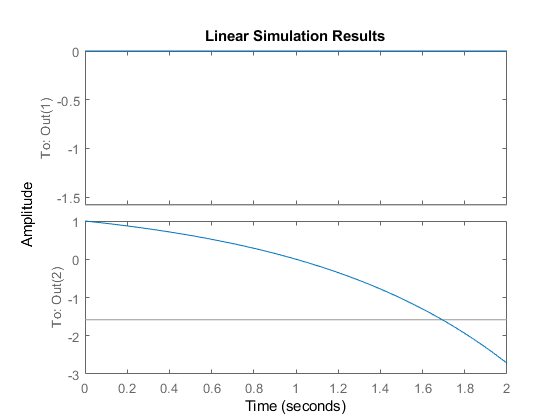
\includegraphics[width=\textwidth]{q6.png}

\end{document}
